% !TeX program = lualatex
% !TeX encoding = UTF-8
% !TeX spellcheck = fr_FR
% !TeX root = main.tex

\documentclass[11pt,a4paper]{article}

\title{Comment l'automatisation peut-elle permettre d'améliorer le cycle de vie d'une application ?}
\author{Sylvain METAYER}

\usepackage{indentfirst}
\usepackage{shellesc,xpatch}
\usepackage[french]{translator}
\usepackage{float}
\usepackage{glossaries} % Pour faire des glossaires
\usepackage{natbib} % Pour créer des références bibliographiques
\usepackage{comment} % Pour les commentaires
\usepackage{graphicx} % Pour les images
\usepackage[french]{babel} % Document FR
\usepackage[T1]{fontenc} % Document FR
\usepackage{fontspec} 
\usepackage{fancyhdr} % Pour des en-tête et pied de page stylé
\usepackage{url} % Pour afficher les URL
\usepackage{appendix} % Pour les annexes
\usepackage{listings} % Pour les tables de code.
\usepackage{eso-pic}
\usepackage{wrapfig}
\usepackage{todonotes} % Pour les TODO
\usepackage{xcolor} 
\usepackage[cache=false]{minted} % Pour afficher du code proprement. Besoin de rajouter cache=false pour corriger un bug dans minted
\usepackage[normalem]{ulem} 
\usepackage{enumerate} % Des listes numérotées.
\usepackage{pdfpages}
\usepackage{epigraph}

\usepackage{lipsum} % only for demonstrating purpose, you can safely remove this package
%% \lipsum
%% \lipsum[3-56] 

\usepackage{tikz}
\usetikzlibrary{calendar}
\usepackage{placeins}
\usepackage{textcomp}
\usepackage{pgfgantt}


% Définitions des titres
\renewcommand\listoflistingscaption{Liste des codes sources}
\renewcommand\listingscaption{Code}

% pour switch auto papier / pdf
\newtoggle{paper}

% Pick one and comment the other one.
% \toggletrue{paper}
\togglefalse{paper}

\iftoggle{paper}{%
	% paper
	\usepackage[left=6cm,right=4cm,top=4cm,bottom=4cm]{geometry} % Pour le rapport imprimé 
}{%
	% electronic
	\usepackage[left=3cm,right=3cm,top=3cm,bottom=3cm]{geometry}
}

% Gestion des marges. Lien utile.
% https://www.debian-fr.org/t/latex-definir-un-paragraphe-en-dehors-des-marges/13991/3

% Réglages d'affichage
\setcounter{tocdepth}{3} % granularité de la table des matières
\setlength{\parindent}{3em} % On modifie l'indentation des paragraphes
\setlength{\parskip}{1em} % On modifie l'espace entre les paragraphes
\widowpenalty=10000 % Pour les veuves et les orphelines
\clubpenalty=10000 % Pour les veuves et les orphelines
\FrenchFootnotes %% FROM : http://www.xm1math.net/doculatex/notesbasdepage.html
\newcommand{\numerotationType}{arabic} %Type de numérotation : Roman ou arabic

%% FROM http://forum.mathematex.net/latex-f6/glossaire-t8654.html#p85429
\renewcommand{\glstextformat}[1]{#1*} % Affichage dans le corps du texte d'une entrée du glossaire


%%%%%%%%%%%%%%%%%%%%%%%%%%%%%%%%%%%%%%%%%%%%%%%%%%%%%%%%%%%%%%%%%%%%%%%%%%%%%%%%%%%%%%%%%%%%%%
\begin{comment}
	Fonction utilisée pour insérer une image. L'image doit être située dans le répertoire "img"
	Paramètres : 
	#1 : Positionnement de l'image [Paramètre optionnel]
			H 	Place le flottant ici, c'est-à-dire à l'endroit auquel il apparaît dans le texte source.
			t 	Position en haut de la page.
			b 	Position en bas de la page.
			p 	Place sur une page particulière réservée aux flottants.
			! 	Passe outre les paramètres internes que Latex utilise pour déterminer une position optimale des flottants. (déconseillé)
	#2 : échelle de l'image
	#3 : nom absolu du fichier (extension du fichier comprise)
	#4 : Commentaire affiché sous l'image
	#5 : id de l'image (utile pour y faire référence par la suite)
	Exemple d'utilisation :
	\newImage{2}{test.png}{ceci est un test}{test} : Laisser LateX se demerder pour placer au mieux
	\newImage[H]{2}{test.png}{ceci est un test}{test} : Forcer le placement de l'image à cet endroit exact.
\end{comment}
\newcommand{\newImage}[5][h]
{
\begin{figure}[#1]
    \centering
    \includegraphics[scale=#2]{img/#3}
    \caption{#4}
    \label{fig:#5}
\end{figure}
}

%%%%%%%%%%%%%%%%%%%%%%%%%%%%%%%%%%%%%%%%%%%%%%%%%%%%%%%%%%%%%%%%%%%%%%%%%%%%%%%
% Same as before, but annexe without captions.
\newcommand{\newImageAnnexe}[4][h]
{
\begin{figure}[#1]
    \centering
    \includegraphics[scale=#2]{img/#3}
    \label{annexe:#4}
\end{figure}
}

%%%%%%%%%%%%%%%%%%%%%%%%%%%%%%%%%%%%%%%%%%%%%%%%%%%%%%%%%%%%%%%%%%%%%%%%%%%%
\begin{comment}
	Fonction utilisée pour ajouter une URL.
	@see http://timmurphy.org/2010/04/04/referencing-website-urls-with-latex-bibtex/ ?
	Paramètres : 
	#1 : url (doit OBLIGATOIREMENT faire référence à un id de main.bib)
	#2 : Nom donné
	Exemple d'utilisation :
	\addURL{www.google.fr}{Google}
\end{comment}
\newcommand{\addURL}[2]
{
#2\footnote{#1 (cf. entrée \cite{#1} des références)}
}

%%%%%%%%%%%%%%%%%%%%%%%%%%%%%%%%%%%%%%%%%%%%%%%%%%%%%%%%%%%%%%%%%%%%%%%%%%%%%
\begin{comment}
	Fonction pour ajouter un acronyme contenant une définition au glossaire.
	Paramètres : 
	#1 : id acronyme
	#2 : Nom acronyme court
	#3 : Nom complet acronyme
	#4 : Description dans le glossaire

	Exemple d'utilisation :
	\newAcronym{API}{API}{Application Programming Interface}{Définition de API}
\end{comment}
\newcommand{\newAcronym}[4]
{
	\newglossaryentry{#1}
	{
			name={#2},
			description={#4},
			first={\glsentrylong{#1} (#2)},
			long={#3}
	}
}

%%%%%%%%%%%%%%%%%%%%%%%%%%%%%%%%%%%%%%%%%%%%%%%%%%%%%%%%%%%%%%%%%%%%%%%%%%%%%%%%%%%%%%%%%%%%%%
% http://www.developpez.net/forums/d961640/autres-langages/autres-langages/latex/mise-forme/referencer-annexe/#post5400726
% Pas un grand intérêt, mais à garder sous le coude, on sait jamais.
\newcommand{\annexe}[1]{annexe~\ref{#1} (page~\pageref{#1})}
%%%%%%%%%%%%%%%%%%%%%%%%%%%%%%%%%%%%%%%%%%%%%%%%%%%%%%%%%%%%%%%%%%%%%%%%%%%%%%%%%%%%%%%%%%%%%%
\begin{comment}
	Quelques commandes utiles pour la compilation avec un index ou des références.
	
	Build Glossaries
		- "makeindex.exe -s main.ist -t main.glg -o main.gls main.glo"
	
	Build References
	- "bibtex main"
	
	Exemple bibliographie dans le fichier main.bib :
	\@Misc{ 
		google, % Identifiant pour y faire références
		note = {}, % Une note optionnelle
		title = {Google}, % Titre
		author = {\url{google.com}} % Lien vers URL ou titre du livre.
	}
	
	Créer des tableaux LateX facilement
	http://www.tablesgenerator.com
	
\end{comment}

%%%%%%%%%%%%%%%%%%%%%%%%%%%%%%%%%%%%%%%%%%%%%%%%%%%%%%%%%%%%%%%%%%%%%%%%%%%%%%%%%%%%%%%%%
% This is where the magic happens..
\newcommand{\nocontentsline}[3]{}
\newcommand{\tocless}[2]{\bgroup\let\addcontentsline=\nocontentsline#1{#2}\egroup}

% Définir le titre des annexes dans le sommaire (ne marche pas si mis dans parameters)
\renewcommand{\addappheadtotoc}{Annexes}


% Création glossaire
\makeglossaries
% Chargements des entrées du glossaire. APRES \makeglossaries
\loadglsentries{glossaire.tex}
\addbibresource{main.bib}

% Début du document
\begin{document}
	\selectlanguage{french}
	\pagestyle{plain} % Juste le numero de page pour en-tête / pied de page.
	\pagenumbering{gobble} % pas de numérotation
	%%%%%%%%%%%%%%%%%%%%%%%%%%%%%%%%%%%%%%%%%
% University Assignment Title Page 
% LaTeX Template
% Version 1.0 (27/12/12)
%
% This template has been downloaded from:
% http://www.LaTeXTemplates.com
%
% Original author:
% WikiBooks (http://en.wikibooks.org/wiki/LaTeX/Title_Creation)
%
% License:
%% CC BY-NC-SA 3.0 (http://creativecommons.org/licenses/by-nc-sa/3.0/)
% 
% Instructions for using this template:
% This title page is capable of being compiled as is. This is not useful for 
% including it in another document. To do this, you have two options: 
%
% 1) Copy/paste everything between \begin{document} and \end{document} 
% starting at \begin{titlepage} and paste this into another LaTeX file where you 
% want your title page.
%% OR
% 2) Remove everything outside the \begin{titlepage} and \end{titlepage} and 
% move this file to the same directory as the LaTeX file you wish to add it to. 
% Then add \input{./title_page_1.tex} to your LaTeX file where you want your
% title page.
%
%%%%%%%%%%%%%%%%%%%%%%%%%%%%%%%%%%%%%%%%%

\begin{titlepage}

\newcommand{\HRule}{\rule{\linewidth}{0.5mm}} % Defines a new command for the horizontal lines, change thickness here

\center % Center everything on the page
 
%----------------------------------------------------------------------------------------
%%	HEADING SECTIONS
%----------------------------------------------------------------------------------------
\begin{minipage}{0.4\textwidth}
	\begin{flushleft} \large
		EPSI Bordeaux\\
		114 Rue Lucien Faure\\
		33000 Bordeaux
	\end{flushleft}
\end{minipage}
~
\begin{minipage}{0.4\textwidth}
	\begin{flushright} \large
		\onepoint\\
		28 Avenue Léonard de Vinci \\
		33600 PESSAC
	\end{flushright}
\end{minipage}\\[2cm]


\textsc{\LARGE EPSI Bordeaux - 5\up{ème} année}\\[1.0cm]

\space

\HRule \\[0.4cm]
{ \huge \bfseries 
Comment l'automatisation peut permettre de réduire les erreurs humaines dans la mise en oeuvre d'une application ?
}\\[0.4cm]
\HRule \\[1.5cm]

\LARGE Sylvain \textsc{METAYER}\\[2cm] % Your name

\begin{flushleft} \large
	\emph{Tuteur Entreprise :}\\
	Nicolas \textsc{GUERINET}
	\newline\newline
	\emph{Tuteur EPSI :} \\
	Sylvain \textsc{LABASSE}
\end{flushleft}


\includegraphics[scale=0.2]{img/epsi.png}\\[1cm] % Include a department/university logo - this will require the graphicx package


\includegraphics[scale=0.05]{img/onepoint.png}\\[1cm] % Include a department/university logo - this will require the graphicx package

\begin{flushright} \large 
	Promotion 2019, Soutenu en Septembre 2019
\end{flushright}

\vfill % Fill the rest of the page with whitespace

\end{titlepage} 
\newpage
	~ % Hide summary page.
\newpage
	%% TODO Listing. Add disable option to package before printing !
	\iftoggle{todoExplain}{%
		\section*{Détails des couleurs todo}
		\begin{itemize}
			\item \emph{gray} est utilisé pour les parties obligatoires, mais non relative au contenu pur du mémoire (remerciements, abstract...)
			\item \emph{red} est utilisé pour les todos nécessitant de la recherche et de la rédaction.
			\item \emph{orange} est utilisé pour les parties nécessitant des refonte, soit sur la forme, soit parce qu'elle doivent être liées à d'autres parties.
			\item \emph{cyan} est utilisé pour les parties nécessitant de la rédaction sans recherche.
			\item \emph{yellow} est utilisé pour des estimations de nombre de page que la partie est \emph{censée} occuper.
		\end{itemize}
	}{}
	\listoftodos 
\newpage
	\section*{Remerciements}
	\todo{Remerciement, 1 page}
\newpage
	\shorttoc{Sommaire}{2} % Only sections
\newpage
\newpage
	\pagenumbering{\numerotationType} % start numerotation
	
\includepdf[scale=0.8,pagecommand=\section*{Attestation de non plagiat}, offset=0 -2cm]{docs/non-plagiat.pdf}
	\addcontentsline{toc}{section}{Attestation de non plagiat} % ajout de la référence dans la table des matières
\newpage
	\section*{Résumé}
	\addcontentsline{toc}{section}{Resumé} % ajout de la référence dans la table des matières
	\todo[color=gray]{Résumé de 2-3 pages en français.}

\begin{abstract}

{\em
Ce document est réalisé à l'aide de \LaTeX. La dernière version de ce document, ainsi que ses sources, sont disponible à l'adresse suivante.

\centerline{\url{https://memoire.epsi.sylvainmetayer.fr}}

Pour information, tout mot suivi du symbole \frquote{*} indique une référence vers le glossaire présent page \pageref{glossaire}. Les numéros entre crochets \frquote{[1]} indique une référence vers un élément de la bibliographie disponible page \pageref{bibliographies}
}

\hrulefill
\end{abstract}

\newpage
	\section*{Abstract}
	\addcontentsline{toc}{section}{Abstract} % ajout de la référence dans la table des matières
	% !TeX spellcheck = en_GB

\begin{otherlanguage}{english}
\begin{abstract}


\begin{large}

{\em
	This document is made with \LaTeX. The latest version of this document, along with its source code, can be found at the following website.

	\begin{center}
		\url{https://memoire.epsi.sylvainmetayer.fr}
	\end{center}

	Every words followed by the \frquote{*} symbol indicates a reference to the glossary available at page \pageref{glossaire}. Every number surrounded by brackets \frquote{[1]} indicates a reference to an element of the bibliography available at page \pageref{bibliographies}
}

\hrulefill

The goal of this document is to show you the advantages and tools to implement a \devops{} and automation approach inside an informatic project. Despite the fact that this document has a technical part, it is meant to be read by all people wishing to read it.

This document will start with an history of automation, to install a context of this document. It will then detail each part inside the lifecycle of an application. This will allow the reader to have an overview of the lifecycle of an application.

We will the talk about a practical case, demonstrating the impact of implementing a \devops{} and automation approach with one company, \etsy. This will show the tools and changes made by the company to perform its transition to a \devops{} approach and set up automation processes. We will also talk about the difficulty to set up such a system and why deployments or developments became more complex over time.

In the end, we will get into the concret part of the subject with the way to set up automation approach, from different perspective : organizational, financial, technical alongs with the prerequisite of such an approach

\end{large}

\end{abstract}
\end{otherlanguage}

\newpage
	\section*{Introduction}
	\addcontentsline{toc}{section}{Introduction} % ajout de la référence dans la table des matières
	\todo{Introduction, 5-6 pages}

\todo{Quand la partie introduction sera terminée, supprimer les parties.}

\subsection{Accroche}
L'automatisation a toujours été perçue comme un moyen de gagner en productivité, temps, et donc de rendre des projets toujours plus rentable.
	
Les projets informatiques sont de plus en plus nombreux, que cela soit des logiciels de bureau, des applications web, ou encore avec les nouveaux terminaux, des applications mobile, tablettes ou même pour montres connectées.
	
Les projets augmentent donc en quantité, mais augmentent-ils en qualité ? Leur fiabilité n'est en effet pas toujours optimale. 
	
Combien de projet sont encore déployé manuellement car aucune automatisation n'est présente sur le projet ? 
	
En plus d'une perte de temps, parfois importante, cela engendre un stress au niveau des équipes de développeurs, qui à chaque livraison redoute les régressions qui pourraient survenir ou encore les bugs de déploiement.

L'automatisation peut également permettre d'améliorer l'arrivée d'un nouveau développeur sur un projet. Il n'est en effet par rare de voir des projets ou la configuration de l'environnement requiert à elle seule plusieurs jours, sans que le développeur puisse vraiment commencer à travailler.
	
L'automatisation va permettre d'améliorer la fiabilité ainsi que la confiance des développeurs et clients dans le projet, puisque des tests automatisés ainsi qu'une chaine d'industrialisation complètement automatisée permet ainsi de déployer avec confiance une application.
	
Nous allons donc tenter de répondre à la problématique suivante :
	
{\LARGE \problematique}

\subsection{Définition}

Avant de continuer, il convient de s'attarder sur ce qu'est l'automatisation.

Selon le Larousse, l'automatisation est le 

\begin{quote}
fait d'automatiser l'exécution d'une tâche, d'une suite d'opérations...
\end{quote}

\subsection{Historique}

Idées : 
	
- Mode opératoire suivi religieusement, 

- script expect

- Comment déployait-on avant ?

-  ...


\textit{L’introduction doit remplir une fonction traditionnelle : délimiter et présenter le projet ou la mission et son contexte professionnel, annoncer les parties principales du développement. L’introduction représente environ un dixième du mémoire. Il faut absolument insister sur la bonne impression qu’elle doit donner au lecteur comme premier et décisif contact avec le mémoire.}

\subsection{Que peut-on automatiser ?}

\subsection{Pourquoi automatiser ?}

Quels en sont les avantages ?

- éviter erreurs développeur

- éviter script executé avec mauvais parmaètres

\subsection{Présentation entreprise / mission}

L'entreprise dans laquelle j'effectue mon alternance depuis septembre 2017 est \onepoint. 

\xmakefirstuc{\onepoint{}} est une \gls{esn} à taille humaine. Son domaine d'activité est d'accompagner ses clients dans leur transformation numérique, 

C'est une \gls{SAS} disposant de 14 implantations dans le monde. L'entreprise a effectué en 2018 un chiffre d'affaire de 300 million d'euros.

Elle dispose de 2300 collaborateurs, en moyenne agé de 33 ans.

\xmakefirstuc{\onepoint{}} se compose de plusieurs communautés.

\begin{itemize}
	\item Des communautés \emph{régions}, permettant de regrouper les collaborateurs par leur proximité géographique.
	\item Des communautés \emph{expertise}, regroupant l'expertise de chacun, et permettant à tous de progresser. On y retrouve par exemple la communauté Sécurité ou encore Architecture.
	\item Des communautés \emph{support}, tel que la \gls{DSI}, ou les Ressources Humaines, nécessaire au fonctionnement de l'entreprise.
	\item Des communautés \emph{métiers}, regroupant des personnes maitrisant les aspects métiers des différents clients, ainsi que les contraintes de ces métiers. Cela peut par exemple être les métiers des Assurances, des Banques, des Télécoms... 
\end{itemize}

Ainsi, lors du développement d'un projet, toutes ces communautés sont utilisés, afin de tirer le meilleur d'entre elle et de regrouper les personnes les plus aptes à réaliser le projet.

Cela implique aussi que chaque collaborateur peut ainsi appartenir à une ou plusieurs communautés, selon ses compétences, expérience et localisation.

\subsubsection{Historique} 

\xmakefirstuc{\onepoint{}} a été créé en 2002, par David Layani.

De 2003 jusqu'en 2007, elle va s'ouvrir à l'international, avec l'ouverture de bureaux au Canada, en Chine et en Tunisie.

En 2008, elle étend sa position en France, avec l'ouverture de deux centres de production, à Bordeaux et Nantes.

En 2015, \onepoint{} continue son développement international au Luxembourg, en Belgique et en Hollande, avant de racheter VisionIT Group.

En 2018, \onepoint{} ouvre des bureaux à Lyon et en Australie, et rachète également Weave ainsi que Géronimo, acteur important dans la conception d'application mobile.

\subsubsection{Réalisations}

\subsubsection{Contexte de l'alternance}

Projet Nouvelle Aquitaine, chaine d'industrialisation pour pouvoir permettre déploiement de multiple sites Drupal.

\textit{Projet \bv{}, ou il y a une architecture actuelle qui n'est pas satisfaisante pour X raisons (reproductibilité...), et qui doit être changé}.

\textit{Elaborer un schéma directeur à partir d’orientations stratégiques} => Conduite de changement


\subsection{Annonce du plan}
\newpage
	%%%%%%%%%%%%%%%% FANCY %%%%%%%%%%%%%%%%%
	% Fancy header / footer
	\pagestyle{fancy}
	
	% Obtenir le nom de la section/sous-section sans le numero
	\renewcommand{\sectionmark}[1]{\markright{#1}}
	\renewcommand{\subsectionmark}[1]{\markright{#1}}
	\renewcommand{\subsubsectionmark}[1]{\markright{#1}}
	
	%% HEADER
	%\renewcommand{\headrulewidth}{0.4pt}
	\lhead{\fancyplain{}{}}
	\chead{\fancyplain{}}
	\rhead{\fancyplain{}{\rightmark}}
	
	%% FOOTER
	%\renewcommand{\footrulewidth}{0.4pt}
	\lfoot{\fancyplain{}{}}	
	\cfoot{\fancyplain{}{}}	
	\rfoot{\fancyplain{}{\thepage}}
	%%%%%%%%%%%%%%%% END FANCY %%%%%%%%%%%%

  \section{Cycle de vie d'une application}
	\todo{Cycle de vie d'une application, 8 pages}

Une application, qu'il s'agisse d'une application web ou de bureau se décompose la plupart du temps en plusieurs étapes. Rare, pour ne pas dire quasi-inexistant, sont les projets réussis qui ont été développé sans jalons, sans documentation (bien rédigée ou non), et sans support (technique, utilisateur).

Une application nait du fait de répondre à un besoin. Par exemple, Blablacar\footnote{\url{https://blablacar.fr/}} est né du besoin de répondre à la demande de covoiturage pour se déplacer plus facilement et à moindre coût.

De plus, selon les différentes phases du projet, plusieurs personnes vont être amenées à travailler sur ce dernier. Il est donc primordial de pouvoir établir un suivi de l'application, car si plusieurs personnes interviennent sur un projet, il est tout à fait possible que des personnes aillent et viennent, nécessitant une bonne organisation pour éviter de tout reprendre de zéro à chaque fois.

On peut donc distinguer plusieurs étapes dans le cycle de vie d'une application.

Le but de cette partie est donc de présenter, étape après étape, ces phases.

\todo{Ca serait bien que l'intro de la partie 1 fasse une page au lieu de à peine une demie-page}


\subsection{Répondre à un besoin}

Tout d'abord, avant de développer une application, il s'agit d'exprimer le besoin auquel elle doit répondre. Il s'agit de la première étape, \emph{l'expression du besoin}. Le but de cette étape est de déterminer si le besoin de l'application est réel, à qui est destinée l'application, et de constituer une première équipe qui portera ce projet.

Ainsi, on va d'abord commencer par savoir à quel besoin répondre. Pourquoi cette idée pourrait-elle fonctionner ? Qu'est ce qui fait que cela peut être rentable, ou même utile ? Il est nécessaire de se poser toute ces questions lorsque l'on commence à réfléchir à une idée d'application. 

L'une des premières étapes, peut être est de vérifier si une application similaire, ou répondant déjà à ce besoin n'existe pas déjà. Dans le cas ou une application similaire existe déjà, on peut tenter de se démarquer, en proposant des fonctionnalités supplémentaire, une interface améliorée... Ou parfois tout simplement en utilisant le produit existant et en passant à une autre idée.\footnote{Chaque idée ne débouche pas forcément sur un produit fini, il faut souvent persévérer pour trouver une bonne idée et se démarquer !}

Il s'agit ensuite de déterminer son but, le besoin auquel le produit répond. Par exemple, les VTC\footnote{voiture de transport avec chauffeur} répondent à un besoin de déplacement instantané d'un point A à un point B et une facilité de réservation (le plus souvent via une application, avec géolocalisation des VTC les plus proches).  

De plus, il faut également se renseigner sur les utilisateurs potentiels avant de lancer son produit. Si des services similaires existent, il est nécessaire de pouvoir déterminer une tranche d'utilisateurs à viser. Si le service est nouveau, il faut pouvoir déterminer les \gls{earlyadopter} du service. Cela peut se faire au travers de démonstration d'une version bêta du site, par un sondage en ligne afin de déterminer les cibles les plus à même d'utiliser le service... \todo{Je suis sur qu'on a eu un cours / une ressource sur les early adopter ?}. Pour bien déterminer ses \gls{earlyadopter}, on peut se poser les questions suivantes afin de déterminer des \glsplural{persona} : 

\begin{itemize}
	\item Quel est l'age de la personne ciblée ?
	\item Quel est le métier et la catégorie socio-professionnelle de la personne ciblée ?
	\item Quel est le sexe de la personne cibleé ? 
	\item Ou habite la personne cible ? En ville, en campagne... ? 
	\item Pourquoi a-t-il besoin de ce service ? 
	\item Qu'est ce qui peut l'empêcher d'utiliser le service (aspect financier, lenteur du service...) 
	\item Quel serait un (ou plusieurs) cas d'usage de la personne ciblée avec le service?
	\item ...
\end{itemize}

Une fois la cible établie, il convient également de savoir si la solution est viable financièrement. En effet, on peut avoir la meilleure idée du monde, mais si on ne peut gérer la partie financière du projet, ce dernier est voué à l'échec. Cette étude financière va inclure une étude sur le temps de développement d'une première version, les coûts de communication, des serveurs, des déplacements (forums, congrès...) pour présenter l'application... De l'autre côté, on va déterminer les recettes de l'application, en estimant les revenus que pourrait générer les \gls{earlyadopter} et les autres utilisateurs, ainsi que les autres sources de revenus potentiels (publicité, crowfounding...). Ainsi, lors de la définition des \gls{earlyadopter} via un sondage en ligne, il n'est pas rare de voir une partie concernant les tarifs que les utilisateurs seraient prêt à dépenser, avec des questions telle que par exemple : 

\begin{itemize}
	\item Quel est le prix minimum sous lequel le service est considéré de mauvaise qualité?
	\item Quel est le prix maximum acceptable pour l'utilisation de ce service?
\end{itemize}

- Étude de faisabilité / concurrence

- Définition des responsables du projet

- Collecte d'information sur la faisabilité / besoin du projet.

- Exemple : location de trottinettes => besoin / études /

%% https://medium.com/@faureguillaume/etude-du-march%C3%A9-des-trottinettes-%C3%A9lectriques-en-libre-service-en-france-et-dans-le-reste-du-monde-36b3370b3f4c avec image de la micromobilité 

\todo{Expression du besoin}

\subsection{Planification}

Une autre étape intervenant en amont du projet est la \emph{planification}. Cette étape est très importante et n'est pas à négliger puisqu'elle va permettre de déterminer des jalons qui définiront les moments clés du cycle de vie du projet.

\begin{itemize}
	\item Les dates des ateliers de définitions du besoin entre équipe de développement et client
	\item Les dates de recette et de pré-production du service
	\item La validation client
	\item Les différentes réunions de suivi du projet 
	\item Son annonce au public
	\item Sa mise en production
	\item ...
\end{itemize}

La planification est également une étape qui sera présente durant tout le cycle de vie de l'application, jusqu’à sa fin de vie. L'organisation du projet passe souvent par l'élaboration d'un \glsplural{gantt} pour représenter de façon graphique les jalons du cycle de vie d'une application.

\newImage{0.4}{gantt.png}{Exemple de \gls{gantt} - source : wikimedia.org}{gantt}

Un \gls{gantt} contient donc les différents jalons du cycle de vie d'une application, mais il est aussi nécessaire de prévoir les éléments pouvant être bloquant. Par exemple, dans le cas de collecte de données utilisateurs afin de réaliser un traitement, il convient de prévoir un délai pour effectuer les démarches auprès de la \gls{cnil}, prévoir un délai de validation du contrat avec les différents prestataires, les délais de réponse au sein de l'organisation afin de valider le projet...

Il convient aussi de définir les fonctionnalités par priorités. En effet, selon les délais impartis, il ne sera peut-être pas possible de voir toutes les fonctionnalités présentes dans la première version. Cela impliquerait un \gls{timetomarket} plus élevé, et donc des risques de voir d'autres concurrents se positionner sur le marché. Il est donc plus prudent de définir les fonctionnalités clés de l'application, et de prévoir les autres fonctionnalités dans les évolutions futures. On peut prioriser les fonctionnalités d'une application en plusieurs catégories.

\begin{itemize}
	\item Les \emph{must-have}. Ce sont les fonctionnalités sans lesquelles l'application n'est pas utilisable. Par exemple, si le service propose des achats, mais que le tunnel d'achat ne gère pas les paiements, il sera impossible de compléter la moindre commande, et par conséquent, le site ne sera pas utilisable.
	\item Les \emph{should have}
	\item Les \emph{could have}
	\item Les \emph{won't have}
\end{itemize}

\todo{Finir la partie planification}

- Définition d'un budget

- Négociation commerciale

- Définition risques juridiques / légaux (GDPR, CNIL...).

- Diagramme de Gant pour organisation projet, avec les grandes deadlines.

- Expression du besoin, rédaction cahier des charges. Objectif : supprimer ambiguité

Cahier des charges :permet de définir charte graphique \& architecture projet. Définit objectif. Poser au clair les besoins et spécificités des demandes. Priorisation. Définit qui a quel rôle? Contient des garanties pour le client (SLA...) \& l'entreprise (fonctionnalités hors scope \& co)

- Définition des priorités : Must, Should, May en vue de réaliser un MVP

Dans le cas d'une méthodologie \gls{cycle_v}, une seule phase de réalisation est faite, avant d'effectuer la validation avec le client. Cette méthodologie était beaucoup utilisée dans les années \todo{Chercher les années ou était utilisé Cycle en V}, mais avant l'inconvénient de provoquer une différence entre ce que le client souhaitait réellement et ce qu'il obtenait à la fin, plus ou moins conforme au cahier des charges. 

\newImage{0.5}{gestionProjet.jpg}{Gestion de projet, allégorie. Source : https://www.anyideas.net}{gestionProjet} 

Comme le montre l'image \ref{fig:gestionProjet}, souvent utilisée pour illustrer de manière humoristique les potentielles dérives de la gestion de projet, plus le nombre de personnes est important sur un projet et moins la communication est présente, plus les différences d'interprétation peuvent être importante. 

Une deuxième méthodologie de travail a vu le jour dans les années \todo{Chercher date début agilité}, et a pour objectif de combler ce manque de communication, et de faire des retours rapide au client. Dans cette méthodologie, la phase de réalisation est caractérisée sous forme de sprint, qui inclus non pas toutes les fonctionnalités demandées, mais seulement une partie, qui peut-être réalisable dans un temps convenu avec le client. Le but est de développer fonctionnalités par fonctionnalités, et de pouvoir présenter quelques choses de concret au client lors de chaque fin de sprint. Ainsi, à chaque itération, on se rapproche un peu plus de la version finale du produit, et on apporte constamment de la valeur ajoutée au produit.

\todo{Planification}

\subsection{Réalisation}

La réalisation de l'application intervient après la validation du besoin avec le client. Démarre alors la conception de la charte graphique, la réflexion sur les différentes fonctionnalités demandées, ainsi que les réalisations à proprement parler pour concevoir le site. La réalisation peut se dérouler de deux façons différentes.

- Réalisation graphique

- Plusieurs itérations

- Retour client, demande de précisions sur les fonctionnalités

- Développement de tests

\todo{Réalisation}

\subsection{Mise en recette \& Qualification}

- Déploiement en interne de l'application

- Permet de découvrir les premiers bug avec un environnement de production

- Retour sur ce qui était pensé par le client et ce qu'il veut au final (ce bouton, il le veut vraiment la le client en fait ? Ca fait pas très pratique ici..)

- Environnement pré-production / intégration \& co avant mise en production.

\todo{Mise en recette}

- Qualification : le client vérifie la conformité de l’application développée aux spécifications établies.

- Premier contact de l'application avec le client

- Evolution potentiellement lourde ("oh, au final je voulais plutôt ça, ça se fait bien ? Alors qu'il faut 10j pour le mettre en place")

- Potentiellement plusieurs déploiement avant validation finale

\subsection{Mise en production}

- Choix de la date important (ex: Transport, pas 10j avant la rentrée et tous les parents qui renouvellent l'abonnement de leur enfant.)

- Prévoir les imprévus : validation application mobile, propagation dns...

- Formations utilisateurs

- Promotion client du produit.

- Premier déploiement souvent "stressant"

- Besoin de métrique pour pouvoir déterminer le succès de l'application

\todo{Mise en production}

\subsection{Maintenance}

- Correction de bug au fur et à mesure

- Besoin de métrique pour pouvoir déterminer le statut de l'application, ses performances \& eventuels défauts.

- Suivi des logs 

- Système de remontée d'erreur organisée

\todo{Maintenance}

\subsection{Évolution}

Un projet qui n'évolue pas est un projet mort. Ainsi, il est nécessaire pour une application de se remettre continuellement en question, de chercher et d'implémenter de nouvelles idées, de faciliter la vie de l'utilisateur, de proposer de nouvelles fonctionnalités, de se mettre à jour vis à vis des dernières évolutions technologiques.

\todo{Evolution}

- Vie du projet

- Audit de sécurité, pour se tenir à jour

- Audit de performance

\subsection{Fin de vie d'un projet / Décommissionnement}

\todo{Fin de vie d'un projet}

- Remplacement par une autre solution : transfert des données

- Débat légal sur la conversation ou non des données

- Offrir une solution alternative / une possibilité de récupérer ses données pour les utilisateurs.

\missingfigure{Schéma global reprenant les différents étapes du cycle de vie d'une application}
\newpage
	\section{Mise en œuvre une démarche d'automatisation}
	\subsection{Cas pratique}

Maintenant que nous avons vu les différentes étapes qui composaient le cycle de vie d'une application, nous pouvons voir, au travers d'un cas pratique, la mise en place d'une démarche d'automatisation dans un projet ou, dans le cas présent, d'une entreprise.

L'entreprise retenue pour l'étude suivante est \etsy\footnote{\url{https://www.etsy.com}}. \etsy{} est une entreprise créée en 2005 spécialisée dans la vente de création personnelles. Elle permet à ses utilisateurs de créer leurs boutiques et d'y vendre leurs créations à toute la communauté. En 2013, elle comptait plus de 4 millions d'items vendus et disposait d'une communauté de 22 millions d'utilisateurs pour un total de \numprint{80000} boutiques actives sur leur site.

L'entreprise a connu une forte croissance à ses débuts et à donc du s'adapter pour pouvoir offrir une qualité de service et des évolutions constantes.

\subsection{États des lieux}

Avant de détailler la transition effectuée, faisons un état des lieux techniques avant leur transition vers l'automatisation.

\begin{itemize}
	\item \etsy{} dispose d'un environnement \gls{LAMP} et d'une application dite monolithique, c'est-à-dire qu'elle est constituée en une seule partie et donc difficile à faire évoluer lors de grosse mise à jour.
	\item Évidemment, \etsy{} utilisait un gestionnaire de version de son code (\gls{git}) mais n'utilisait pas de branches\footnote{Dans un gestionnaire de version, les branches permettent de séparer les fonctionnalités qui sont en cours de développement ainsi que les différentes versions du code}
	\item Du fait de sa croissance rapide, \etsy{} effectuait 2 à 3 mise à jour par semaine, mais ces dernières étaient effectuées avec difficulté et prenaient environ 4h par livraison. 
\end{itemize}

\epigraph{[deploy were done] twice a week, and each deploy took well over four hours.}{\citetitle{etsyInterview} \cite{etsyInterview}}

Au vu de ces informations et du fait de leur croissance, il était nécessaire de faire évoluer les méthodes de travail et de déploiement pour pouvoir suivre la cadence. L'objectif était donc de passer d'un développement lourd, non organisé à un déploiement rapide permettant un retour rapide sur l'état des déploiements ainsi que plusieurs déploiements par jours.

\todo[color=red]{Cas pratique, 5-6 pages}

a beaucoup utilisé l'open source et y a beaucoup contribué en retour (outil post mortem par ex) %https://github.com/etsy/'

\subsection{Difficulté d'avoir la panacée}

\todo[color=red]{Difficulté d'avoir la panacée, 1-2 pages}

- pourquoi n'existe pas une solution unique ? 

- Pourquoi complexité des processus de déploiement ? 

- chaque outil répond à un besoin, mais existe-t-il un outil all-in-one ? (non)

Solutions existantes

Chef, puppet, ansible, jenkins, travis, docker, terraform, heroku, aws, ...

Combinaison d'outils qui répondent à un besoin, pattern.


\textbf{ATTENTION : NE PAS REPONDRE A LA QUESTION, SEULEMENT SOULEVER DES INTERROGATIONS POUR LE LECTEUR}

Cas pratique (démo entreprise migration) / Comment le généraliser (NE PAS RÉPONDRE A CETTE QUESTION). Cas précis et généraliser, parler des autres solutions. Difficulté d'avoir une solution clé en main, une solution à tout, la panacée

Qu'est ce qui a poussé à l'automatiser ? Complexification de ces étapes (npm) pour pousser à la nécessité l'automatisation. Le fait que l'utilisateur veut toujours plus de simplicité pousse à toujours plus de complexité de réalisation. Permet de se concentrer sur des tâches à forte valeur ajoutée.

Innovation technologique 
\newpage
	\section{Automatisation du cycle de vie}
	\todo{Automatiser un projet}

\subsection{Partie Management, gestion de projet}

Pré-requis, comment gérer la mise en place avec le management, ... Gérer les différentes personnes impliquées, ...

\subsection{Localement, lors des phases de développement}

But : prévenir l'erreur avant qu'elle ne quitte le poste du développeur (et soit donc sur le dépôt Git).

 \begin{itemize}
 	\item Linter
 	\item Docker, stack reproductible et indépendante selon environnement (windows/linux/mac) 
 	\item IDE à configurer, éventuellement partager la configuration (ex: PHP Storm Code Style)
 	\item Makefile / scripts shell de taches récurrentes (cache clear, installation, ...)
 	\item Git hook pour vérifier que tout est ok.
 \end{itemize}

\subsection{Intégration et déploiement continu}

Retour le plus rapide possible pour éviter des bugs en prod. 

Vérifier les dépendances (failles, ...)

le reporting de bug automatique (sentry.io)

Intégration des tests dans gitlab-ci / jenkins

Monitoring : monit pour monitorer l'état d'application ? (perso)

Jenkins, Travis, Déployer automatiquement à partir d'un push sur dev, en recette, intégration, staging, et lorsque tout passe, en production.

\textit{Exemple : parler de \clubSportif Automatisation de la création de la base de données (projet club sportif) et de la restauration des données}


\subsection{L'importance des tests}

Tout l'automatisation ne sert à rien sans une bonne campagne de tests, fonctionnel, unitaire, d'intégration, E2E, ...

Parler de Protractor et Squash sur \bv. Tests automatisés unitaires (phpunit) permettant à la plateforme d'intégration continue de vérifier la conformité du code par rapport aux attentes métier.

différence entre intégration continue et tests unitaire (image du lavabo + séchoir à mains côte à côte). Les test unitaires vont tester la cohérence d'une partie du système tandis que l'intégration va tester la cohérence de l'échange entre divers systèmes / fonctions.

\subsection{Et la sécurité dans tout ça ?}

Gestion des tokens, gestion des comptes.
Un compte admin ou plusieurs sous compte avec des droits limités ? En cas d'intrusion, un attaquant a moins de chance de corrompre tout le système.
Infra : restriction d'accès (htaccess / firewall / ..?)


Attention à l'endroit ou sont fait les builds/tests. Il est préférable, pour des raisons de sécurité évidente d'utiliser un outil auto-hébergé, open source, plutôt que des outils clés en main, ou les données sont envoyées sur des serveurs inconnus. 

Dans certains cas, l'application ne doit pas quitter le périmètre de l'entreprise,il faut donc avoir la maitrise totale de la chaine d'industrialisation
\	newpage
	\pagestyle{plain} % Juste le numéro de page pour en-tête / pied de page à partir de maintenant
	\section*{Conclusion}
	\addcontentsline{toc}{section}{Conclusion} % ajout de la référence dans la table des matières
	\todo[color=yellow]{Conclusion, 7 pages}

- Pourquoi n'existe pas une solution unique ? => car chaque projet différent 

- Pourquoi complexité des processus de déploiement ? => car complexité application en hausse, et demande utilisateur avec toujours plus de simplicité, et donc complexe à réaliser. Passage d'une "application à la bonne franquette", à un vrai processus éprouvé pour durer

\subsection{Bénéfices}

\todo[color=orange]{Benefices}

\textit{dentifier les leviers d’économie à actionner pour améliorer les processus Qualité.}

\begin{itemize}
	\item KPI à trouver
	\item Confiance dans la livraison
	\item ROI avec rapidité de livraison
	\item Décharge l'équipe
	\subitem Plus de temps pour de la valeur métier
	\item L'automatisation peut permettre de relancer rapidement une activité défaillante (SLA / PRA / PCA)
\end{itemize}

\begin{itemize}
	\item - Erreur développeur
	\item + de Fiabilité
	\item Preuve de qualité
	\item Time To Market réduit
	\item Reproductibilité
\end{itemize}

Comment faire en sorte que ça marche dans la durée ? Des controles / supervisons périodique afin de checker que tout va bien.

Workflow : savoir ce qui est automatisé, comment c'est mis en oeuvre ,documentation des outils, ...
Faire en sorte que l'automatisation ne casse pas et que l'on en tire quelques chose, que l'on soit nouvel arrivant sur le projet, ou développeur déjà présent sur le projet.

Scalabilité : Docker / provisionner de nouveaux serveurs rapidement avec Ansible par exemple.

Déploiement : chaine de déploiement (dev/test/inte/preprod/prod) avec chacune ses spécificités

Exemple :

en dev, on souhaite des logs direct dans la console, en prod on les mets dans un fichier de log.
en dev, on veut le mode debug, en prod on le désactive.

\subsection{Limites}

\todo[color=yellow]{Limites}

Sur-qualité, sur-optimisation, ...

Aucun intérêt si les tests ne sont pas fiable.

Dépend du client, de l'environnement, demande de la flexibilité, délai de mise en place, ROI

Pré-requis à l'automatisation

Attention, auto != vérité \url{https://www.matuzo.at/blog/building-the-most-inaccessible-site-possible-with-a-perfect-lighthouse-score/}

L'automatisation ne peut être utilisée, ou sera risquée, ou plus à même d'amener des régression si de mauvaise pratique sont présentes.

\begin{itemize}
	\item variable codée en dur à la place de variable d'environnement
	\item ...
\end{itemize}

De plus, il faut une certaine organisation.

Cela peut-être perçu comme une perte de temps par certaines personnes (hiérarchie, manager, ...), qui y verrons la une perte d'argent et de temps par exemple. Il faut alors pouvoir montrer que cela est rentable, au travers de \gls{KPI} bien déterminé.

Le fait d'automatiser des processus permet de gagner du temps, et par conséquent de l'argent et de consacrer ses efforts à d'autres taches qui peuvent apporter de la valeur métier.

Le coût horaire libéré, calculer à partir de combien de temps il est rentable.

Par exemple, une tache à 3000€ qu'on automatise et qui ne coute plus que 300€ est rentable en 10 semaines.

Facteur humain : Le temps libéré par l'automatisation des tâches peut permettre de souder les liens d'une équipe et d'améliorer les relations de cette dernière. Cela libère du temps pour du team building par exemple.

Un sujet technique qui rapproche en terme d'humain

Idées de \gls{KPI} en vracs.

Métrique - KPI - temps de déploiement / nombre d'incident / uptime / Nombre de build KO / Nombre de build OK ... permettent de définir l'impact des services mis en place sur le S.I

\begin{itemize}
	\item temps de déploiement
	\item taux de déploiement succès
	\item couverture de code
	\item tests au verts
	\item derniers build KO
\end{itemize}

Parler de l'importance de l'implication du client. 

Ex :  Rédaction de SFD, qui évolue tout les 4 matins, et demande un changement dans l'architecture => automatisation perdante.

Dépôt git du mec qui automatise tout \url{https://github.com/NARKOZ/hacker-scripts}

\subsection{Ce qui n'est pas encore automatisé}

\subsection{Les possiblités d'automatisation dans le futur}

\textit{Parler de ce qui n'est pas encore automatisé, et les différentes pistes d'automatisation possible dans le futur.}



\newpage
	\addcontentsline{toc}{section}{Glossaire}
	\glsaddall % ajouter toutes les entrées n'ayant pas encore été citées
	\printglossaries % afficher le glossaire
\newpage
	\addcontentsline{toc}{section}{Références}
	\nocite{*} % Ajout de toutes les références bibliographiques non citées jusqu'à présent.
	%\bibliographystyle{unsrtnat} 
	%\bibliographystyle{babunsrt}
	%\bibliographystyle{apacite}
	% \bibliography{main}{}
	\printbibliography
\newpage
	\addcontentsline{toc}{section}{Liste des figures}
	\listoffigures 
\newpage
	\addcontentsline{toc}{section}{Liste des code sources}
	\listoflistings
\newpage
	\addcontentsline{toc}{section}{Liste des tableaux}
	\listoftables
	\vfill
	\begin{flushright} \large 
		Rédigé avec \LaTeX 
	\end{flushright}
\newpage
	\addcontentsline{toc}{section}{Table des matières}
	\tableofcontents
\newpage
	\addcontentsline{toc}{section}{Annexes}
	\pagenumbering{gobble} % No numérotation
	\vspace*{\stretch{1}}
		\begin{center}
			\begin{Huge}
				\section*{\MakeUppercase{Annexes}} 
			\end{Huge}
		\end{center}
	\vspace*{\stretch{1}}
\newpage
	\appendix % Annexes with A, B, C, D numérotation
	\section{Schéma simplifié du cycle de vie d'un projet}
\newImageAnnexe[H]{0.75}{cycle-vie-projet.png}{cycleVieProjet}

\clearpage
\section{Construction des modules communs de l'application au sein d'un projet \naq}
\newImageAnnexe{0.9}{modules.png}{commons-modules}

\clearpage
\section{Build continu d'un projet \naq}
\begin{figure}[ht]
	\centering
	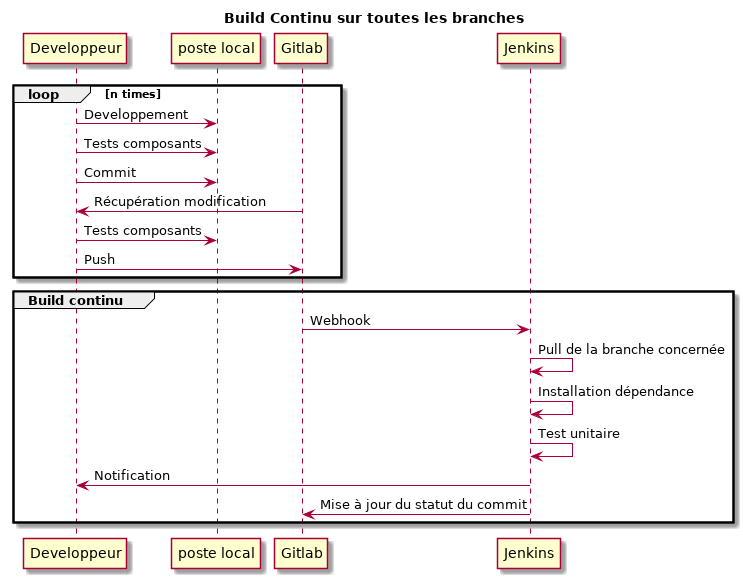
\includegraphics[scale=0.6,angle=-90]{img/build-continu.png}
	\label{annexe:build-continu}
\end{figure}

\clearpage
\section{Flux de travail du déploiement d'une version d'un site \naq}
\newImageAnnexe{0.32}{release.png}{release-naq}

\clearpage
\section{Matrice de développement \devops}

\normalsize{Source : \url{https://www.infoq.com}}

\begin{figure}[ht]
	\centering
	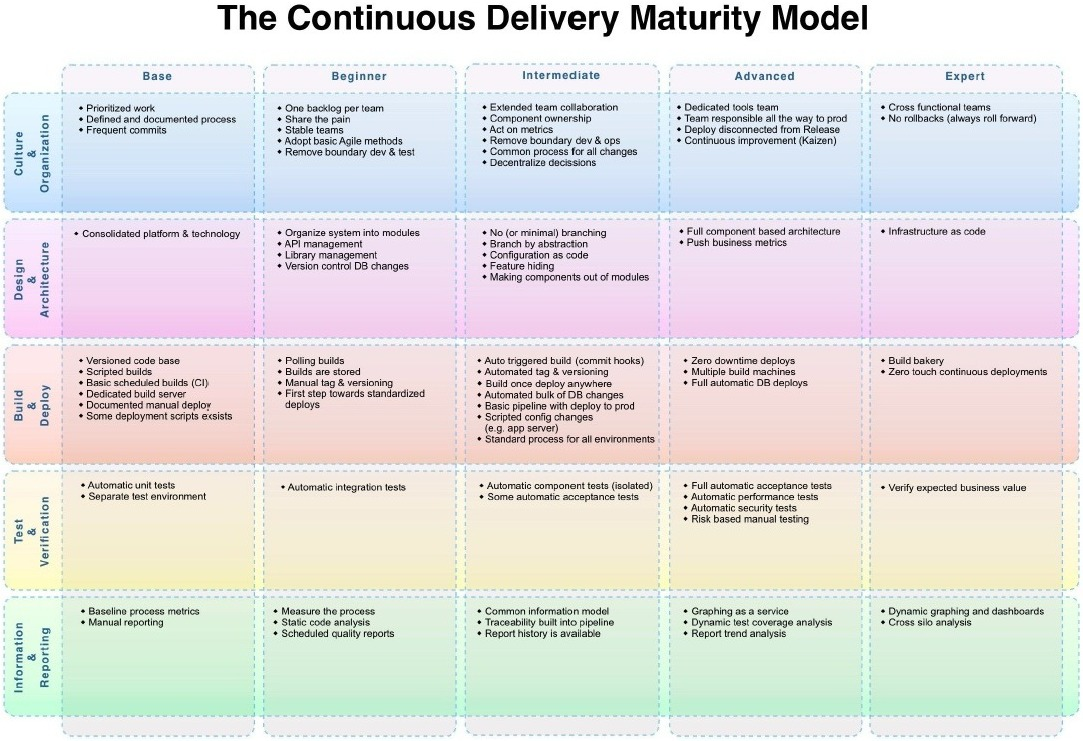
\includegraphics[scale=0.62,angle=-90]{img/devops-matrice.jpg}
	\label{annexe:devops-matrice}
\end{figure}

\clearpage
\section{Exemple d'erreurs détectées par PHPStan}

Dans l'exemple ci-dessous, PHPStan retournera une erreur indiquant que le paramètre requis \frquote{\$type} n'a pas été renseigné, ainsi qu'une erreur indiquant que la méthode privée \frquote{internalBehaviour} ne peut être utilisée en dehors de la classe. 

Il est à noter que cette analyse statique de code peut être et est souvent effectuée au sein de l'\gls{IDE} pour permettre une détection de l'erreur au plus tôt.

\begin{minted}[linenos]{php}
<?php
// index.php

require_once(__DIR__."/vendor/autoload.php");
$a = new \App\File();
$content = $a->loadFile("file.json");
$a->internalBehaviour();

// src/File.php

namespace App;

class File {
  public function loadFile($file, $type) {
    $content = file_get_contents($file);
    if ($type == "json") {
      return json_decode($file);
    }
    return $content;
  }
  
  private function internalBehaviour() {
    echo "this is not public";
  }
}

// ------ ------------------------------------------------------------------- 
// Line   index.php                                                          
// ------ ------------------------------------------------------------------- 
// 6      Method App\File::loadFile() invoked with 1 parameter, 2 required.  
// 7      Call to private method internalBehaviour() of class App\File.      
// ------ ------------------------------------------------------------------- 

\end{minted}
\label{annexe:php-error}


%\clearpage
%\section{Flux de travail pour un hotfix sur un site \naq}
%\newImageAnnexe{0.25}{hotfix.png}{hotfix-naq}
\end{document}
